\documentclass{article}
\usepackage[left=2cm,right=2cm,top=2cm,bottom=2cm]{geometry}
\usepackage[utf8]{inputenc}
\usepackage[german]{babel}
\usepackage{amsmath}
\usepackage{dsfont}
\usepackage[export]{adjustbox}
\usepackage{amsthm}
\usepackage{color}
\usepackage{amsfonts}
\usepackage{amssymb}
\usepackage{wasysym}
\usepackage{makeidx}
\usepackage{graphicx}
\usepackage[colorlinks=true,urlcolor=blue,linkcolor=blue]{hyperref}
\usepackage{ziffer}
\usepackage{minted}
\usepackage{xcolor}
\usepackage{framed}
\usepackage{mdframed}
\usepackage{subfiles}
\usemintedstyle{emacs}

\definecolor{purp}{HTML}{9A72AC}
\definecolor{re}{HTML}{FC6255}
\definecolor{gre}{HTML}{83C167}
\definecolor{blu}{HTML}{58C4DD}
\definecolor{shadecolor}{rgb}{0.85,0.85,0.85}
\definecolor{bg}{rgb}{0.95,0.95,0.95}
\setlength{\parindent}{0em} 

\BeforeBeginEnvironment{minted}{\begin{mdframed}[linewidth =2 ,backgroundcolor=bg , linecolor=black, linewidth=0.5]}
\AfterEndEnvironment{minted}{\end{mdframed}}

\newtheorem{defi}{Definition}
\BeforeBeginEnvironment{defi}{\begin{mdframed}[linewidth =2 ,backgroundcolor=bg , linecolor=black, linewidth=0.5]}
\AfterEndEnvironment{defi}{\end{mdframed}}

\newcommand{\bsp}{\textbf{Beispiel}:}
%\newcommand{\task}{\textbf{Aufgabe}:}

\newcommand{\bol}[1]{\textbf{#1}}
\newcommand{\q}[1]{\glqq #1\grqq}
\newcommand{\DODO}[1]{\textbf{\textcolor{red}{DODO:}} #1 \\ \begin{center}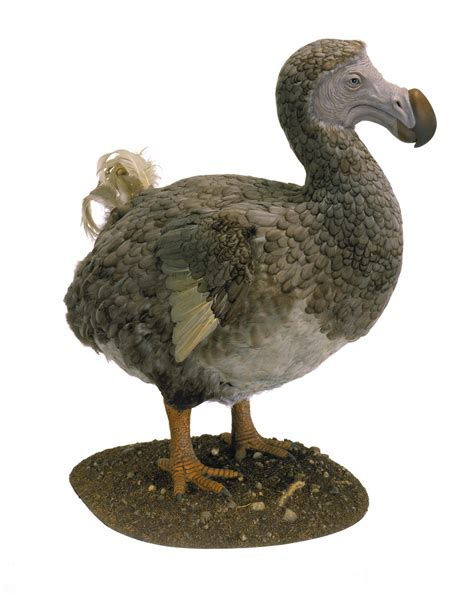
\includegraphics[scale=0.2]{../../media/dodo.jpg} \end{center}}

\newenvironment{task}[1]{
    \begin{shaded*}
    \textbf{Aufgabe #1}:
}{
    \end{shaded*}
}

\begin{document}
\subsection{Grundlagen der Softwaretechnik}
In diesem Kapitel soll es nicht mehr um Projekte gehen, die jeder Einzelne alleine angehen kann, sondern um das \q{Programmieren im Großen} - sei es in einer (internationalen) Firma oder \q{privat} in einem Verbund mit anderen Programmierys. \\
Gerade in großen Projekten ist eine qualitativ hochwertig Zusammenarbeit unerlässlich. Leider gibt es hier immer wieder große Reibungsverluste, neben den fachlichen Inhalten ist die Fähigkeit des \q{Teamwork} - gerade heutzutage - ein immens wichtiger \q{soft skill}. \\
In der Informatik gibt es verschiedene Modelle, die die Projektorganisation strukturieren und z.T. veranschaulichen sollen (dazu gibt es ganze eigene Vorlesungen im Bereich der \textbf{Softwaretechnik}!). \\
Im Allgemeinen geht man grob von den folgenden Phasen im Leben eines Softwareprojekts aus:
\begin{enumerate}
    \item \textbf{Anforderungen und Spezifikationen}
    \item \textbf{Planung}
    \item \textbf{Entwurf und Design}
    \item \textbf{Implementierung und Integration}
    \item \textbf{Betrieb und Wartung}
    \item \textbf{Stilllegung}
\end{enumerate}
Zur Beschreibung dieser Phasen, deren Interaktion und zeitlicher Abfolge gibt es verschiedenste Vorgehensodelle, von denen in folgenden Kapiteln einige vorgestellt werden sollen. \\
Zunächst aber noch Details zu den einzelnen Phasen \\
\subsection{Der Lebenszyklus von Software}
\textbf{Anforderungen und Spezifikationen} \\
Grundlegende Fragen, die eine Anforderungsanalyse zu Beginn eines Projektes beantworten sollte, sind z.B.:
\begin{itemize}
    \item welches Problem soll konkret gelöst werden?
    \item welche Leistung soll das geplante Projekt erbringen?
    \item welche Personen müssen mit einbezogen werden?
    \item gibt es sich widersprechende Anforderungen verschiedener Personen/Gruppen?
\end{itemize}
Insbesondere die letzten beiden Punkte sollen verdeutlichen, dass gerade aus Kundensicht nicht immer Einigkeit über den Funktionsumfang oder die genauen Spezifikationen eines Programs herrscht. Eine genaue Spezifikation der zu erbringenden Leistung ist deshalb wichtig, um Unzufriedenheit diesbezüglich vorzubeugen. \\
Die Anforderungsanalyse beschränkt sich aber nicht nur auf konkrete Funktionalität, sondern bildet ein ganzes Spektrum an Faktoren ab:
\begin{itemize}
    \item \textbf{Funktionale Anforderungen}: das was man zunächst erwarten würde - welche Funktion soll das System haben, wie soll es sich verhalten, etc. 
    \item \textbf{Nichtfunktionale Anforderungen}: hier geht es eher um den eigentlichen Betrieb der Software, wie leistungsfähig soll sie sein - d.h. wie groß sind die Anforderungen an Speicher/Prozessor im laufenden Betrieb, ist die Software skalierbar, etc. 
    \item \textbf{Designbedingungen}: gibt es bereits weitere technische Bedingungen, das könnte z.B. bereits existierende Software sein, zu der Schnittstellen vorhanden bzw. eine Kompatibilität hergestellt werden muss. 
    \item \textbf{Prozessbedingungen}: dies sind eher interne Anforderungen der Entwickler - wie viele Personen sind notwendig, wie soll die Vorgehensweise bei der Entwicklung sein (zwar intern zu sehen, aber insbesondere auch der Kontakt mit dem Kunden - Ablieferung eines \q{fertigen} Produkts oder Zwischenstände z.B.). 
\end{itemize}
Übliche Verfahren, die zur Ermittlung der Anforderungen verwendet werden sind z.B. Fragebögen, Interviews, Simulationsmodelle, Workshops, etc.  \\
Die Ergebnisse müssen natürlich verschriftlicht werden, der Auftraggeber fasst alles im sogenannten \textbf{Lastenheft} zusammen, das möglichst konkret die Gesamtheit aller Anforderungen beschreibt - kurz gesagt: \textbf{Was soll erstellt werden?}. \\
Das \textbf{Pflichtenheft} dagegen beschreibt - ebenfalls möglichst konkret - wie der Auftragnehmer die Anforderungen des Auftraggebers lösen möchte, kurz: \textbf{Wie und womit wird umgesetzt}. Erst nach Akzeptanz des Pflichtenhefts beginnt die eigentliche Umsetzung. \\
\textit{Hinweis:} Diese Beschreibung entspricht in der Realität natürlich nicht immer den Gegebenheiten, sondern eher eine etwas akademische Sicht auf die Dinge. Gerade Software-Entwicklung ist ein sehr dynamischer Prozess und lässt sich selten gut in statische Kategorien verpacken. Die Schule kann hier kein sicheres, aktuelles Bild vermitteln, da Regeln und Abläufe ggf. in den Betrieben bereits überholt sind $\Rightarrow$ Praktika deutlich nützlicher, um zu lernen \q{wie der Hase läuft}. \vspace{3mm} \\
\textbf{Projektplanung} \\
In jedem Fall muss es eine Form von \textbf{Projektmanagement} geben, dass das Projekt zunächst inital plant und die \q{Arbeit verteilt}. Spätestens hier muss man sich für ein Vorgehensmodell (siehe nächste Kapitel) entscheiden. Grob könnte man dabei folgende Unterteilung treffen:
\begin{enumerate}
    \item Sind sehr detaillierte Informationen zu den Anforderungen bekannt, bzw. gibt es keine Möglichkeit die Software \q{laufend anzupassen} (man denke z.B. an Flugzeugsoftware, die doch lieber gleich von Anfang an vollständig laufen sollte), so sind eher plan-getriebene, starre Verfahren wie das \textbf{Wasserfallmodell} oder \textbf{V-Modell} notwendig. 
    \item Sind die Informationen dagegen eher vage, der Auftrag ungenau oder eine hohe Flexibilität allgemein gefordert (da bereits wahrscheinlich ist, dass sich Anforderungen im Laufe der Entwicklung verändern), so bieten sich dynamische Modelle an, die sogenannten \textbf{agilen} Ansätze, z.B. \textbf{Scrum}. 
\end{enumerate}
Für Interessierte zum Nachlesen: Instrumente, die die Projektplanung beschreiben sind z.B. \textbf{Gantt-Diagramm}, \textbf{CPM-Netzplan}, \textbf{Petri-Netze} \vspace{3mm} \\

\textbf{Entwurf und Design}\\
Hier geht es darum, dass die Entwickler die Rahmenbedingung für die konkrete Umsetzung des Produks festlegen, also z.B.:
\begin{itemize}
    \item Welche Datenflüsse innerhalb (und außerhalb) der Software gibt es.
    \item Welche Algorithmen sollen verwendet oder entwickelt werden. 
    \item Welche Schnittstellen sind notwendig.
    \item Welche Designprinzipien sollen verwendet werden, z.B. objektorientierte Prinzipien wie Abstraktion (Oberklassen), Kapselung, etc. 
\end{itemize}
Zur Verschriftlichung können dabei die \textbf{UML-} Diagramme wie das Klassendiagram, das Sequenzdiagramm, oder viele weitere verwendet werden. (Für Interessierte und alle die Profis in diesem Bereich werden wollen: \q{UML 2 glasklar} gibt einen guten Überblick). \\
Gerade im Kontext des \textbf{Test-Driven-Development} bietet es sich auch an, bereits in dieser Phase Tests zu konzipieren, die die Integration des Systems in bestehende Strukturen testet! \vspace{3mm} \\

\textbf{Implementierung und Integration} \\
In dieser Phase geht es um die konkrete Umsetzung des zuvor beschriebenen, einzelne Komponenten der Software werden implementiert, getestet und danach zu größeren Einheiten zusammengebaut. In der Regel sollte dabei \textbf{gut dokumentiert werden (:))} und nach einer vorher festgelegten standardisierten Form gearbeitet werden. \vspace{3mm}\\

\textbf{Betrieb und Wartung sowie Stilllegung} \\
Dieser Bereich des Lebenszyklus ist für uns aktuell eher uninteressant, da im Projekt (vermutlich?) keine kommerzielle Software entstehen wird. Grundsätzlich muss hier aber natürlich geregelt sein, ob der Auftragnehmer auch in Zukunft die Einsatzfähigkeit garantieren muss (z.B. bei Einführung neuer Betriebssystem o.Ä.) oder generell: wann endet der Support für die Software?


\subsection{Das Wasserfallmodell}

Wie der Name schon suggeriert handelt es sich hier um ein lineares Modell, bei dem - zumindest in der ursprünglichen Variante - alle Phasen der Entwicklung streng sequentiell nacheinander ablaufen. Es gibt für jede Phasse festgelegte Start- und Endzeitpunkte. Die im vorangegangen Kapitel beschriebenen Phasen orientieren sich auch an den Phasen des ursprünglichen Wasserfallmodells bzw. umgekehrt. Man kann hier also von der \q{klassischen Vorgehensweise} sprechen. \\
Eine modernere Variante, die wiederholende Elemente zulässt wird z.B. so dargestellt: 
\begin{center}
    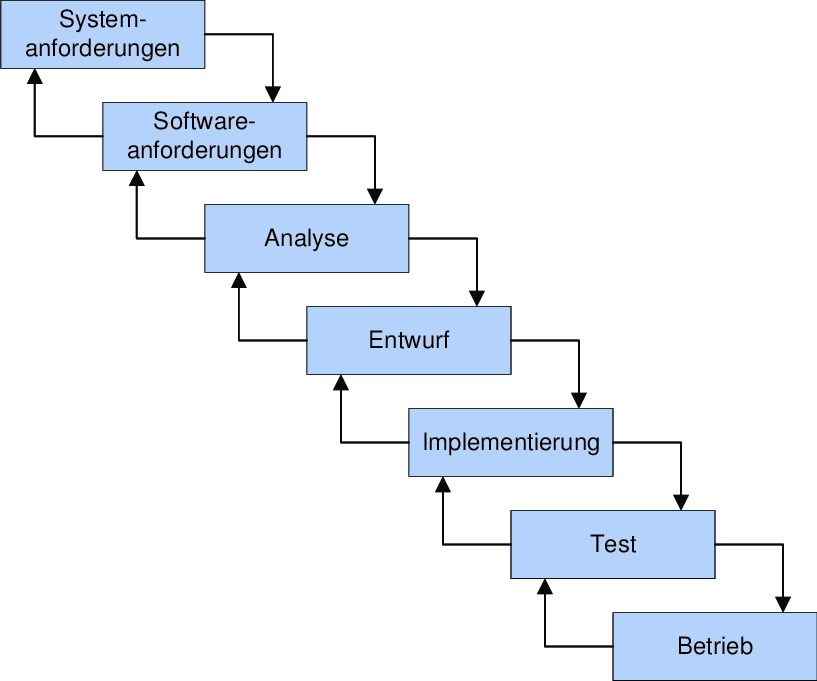
\includegraphics[scale=0.35]{../media/wasserfallmodell.png} \\
    \textit{Quelle:} \href{https://www.researchgate.net/figure/Abbildung-21-Das-Wasserfallmodell_fig1_228914046}{Researchgate}
\end{center}
Damit geht aber der klare Aufbau verloren, für iterative (sich wiederholende) bzw. dynamische Prozesse sind eher die agilen Methoden geeignet.

\subsection{Das V-Modell}

Das V-Modell stellt eine Erweiterung des Wasserfallmodells dar, es handelt sich im wesentlichen aber immer noch um ein lineares Modell:
\begin{center}
    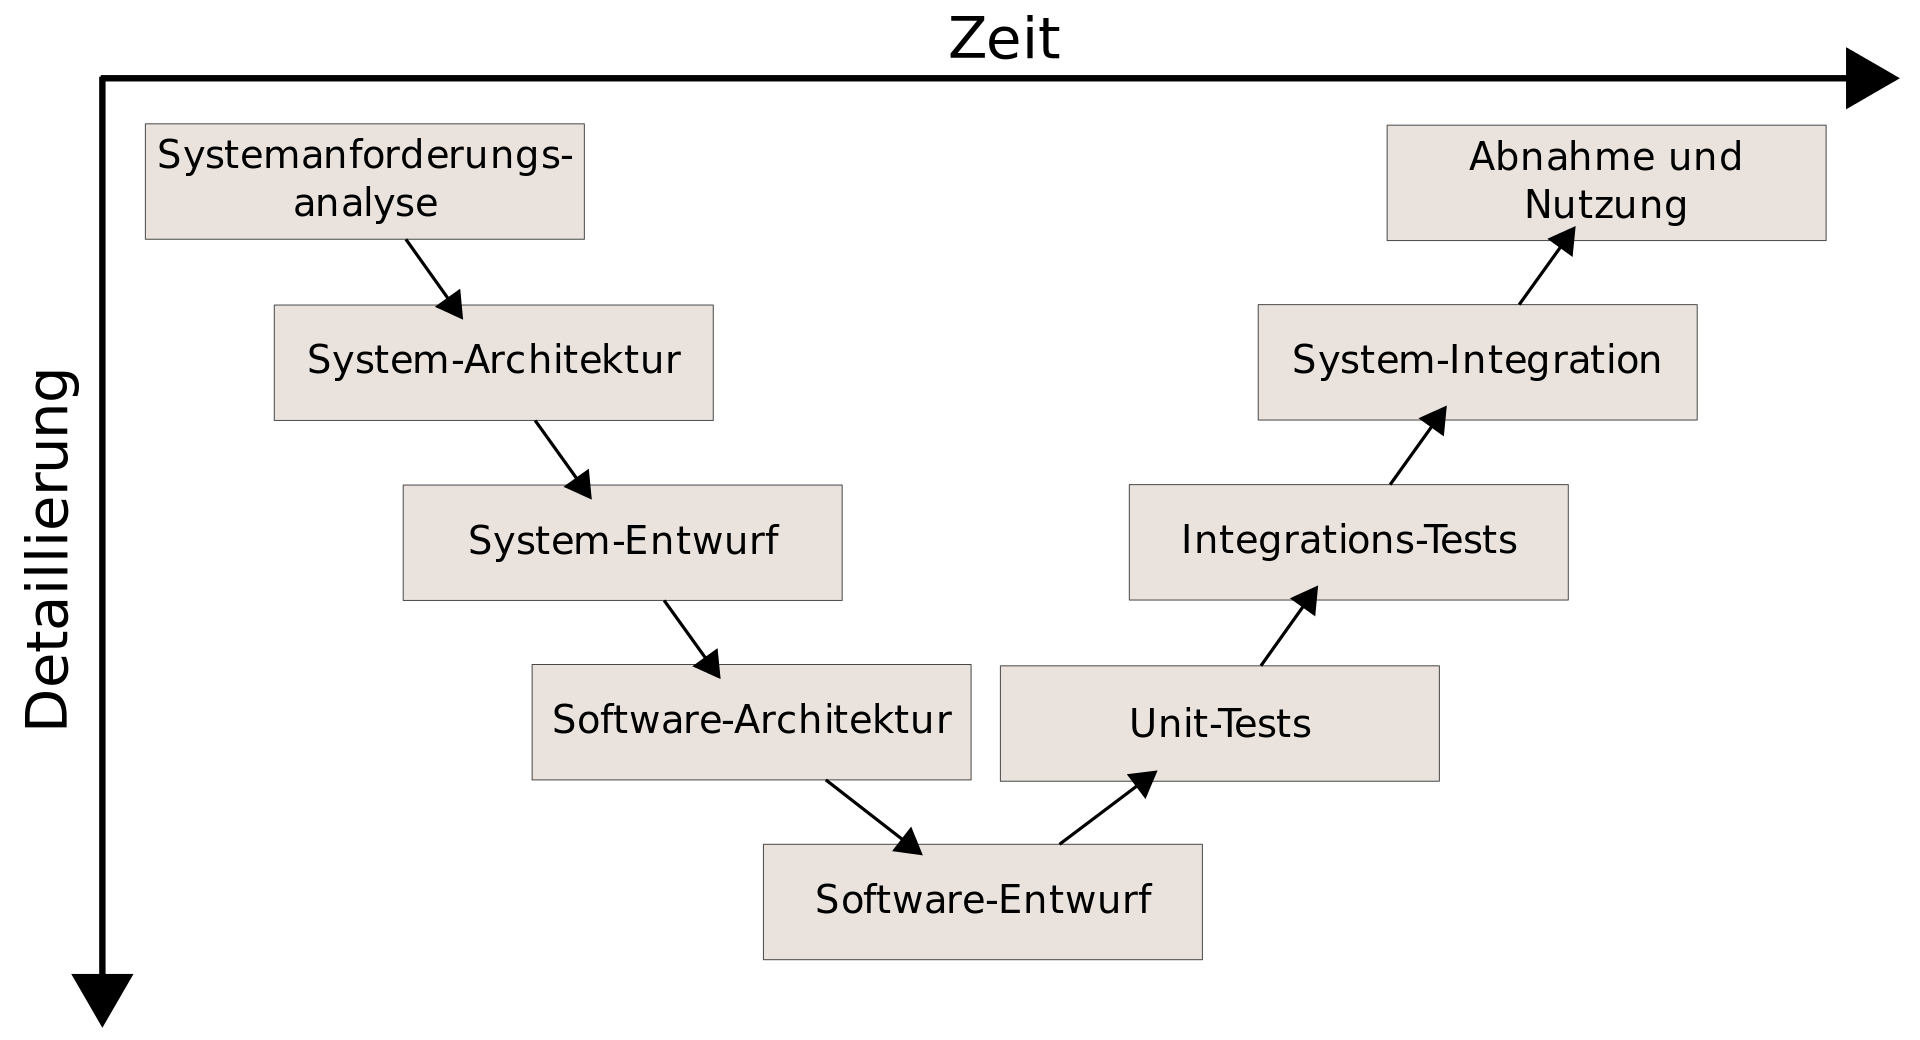
\includegraphics[scale=0.15]{../media/V-Modell.png} \\
    \textit{Quelle:} \href{https://de.wikipedia.org/wiki/V-Modell}{Wikipedia}
\end{center}
Der wesentliche Unterschied zum Wasserfallmodell ist dabei, dass in den einzelnen Ebenen die entsprechenden Tests, die zu diesem Abschnitt gehören, auf der rechten Seite parallel dargestellt werden, d.h. die System-Architektur wird beispielsweise mit System-Integrationstests validiert.

\subsection{Agile Methoden - Scrum}

Die für uns relevanteste Vorgehensmodelle sind die \textbf{agilen Methoden} bzw. \textbf{agile Softwareentwicklung}. Im Gegensatz zu den bisherigen Modellen wird hier die Entwurfsphase möglichst kurz gehalten, d.h. die Entwicklung startet so früh wie möglich. Das bedeutet natürlich, dass die Anforderungen in der Regel nicht vollständig bekannt sind. Das vollständige Lasten- bzw. Pflichtenheft wird dann häufig durch sogenannte \textbf{User stories} ersetzt (siehe Scrum unten). Alle agilen Methoden basieren auf dem \textbf{agilen Manifest} (auch nicht mehr neu: formuliert 2001), eine Zusammenstellung einiger Aussagen, das folgendermaßen lautet: 
\begin{center}
    Wir erschließen bessere Wege, Software zu entwickeln, indem wir es selbt tun und anderen dabei helfen. Durch diese Tätigkeit haben wir diese Werte zu schätzen gelernt:
    \begin{itemize}
        \item \textbf{Individuen und Interaktionen} mehr als Prozesse und Werkzeuge
        \item \textbf{Funktionierende Software} mehr als umfassende Dokumentation
        \item \textbf{Zusammenarbeit mit dem Kunden} mehr als Vertragsverhandlung
        \item \textbf{Reagieren auf Veränderung} mehr als das Befolgen eines Plans.
    \end{itemize}
    Das heißt, obwohl wir die Werte auf der rechten Seite wichtig finden, schätzen wir die Werte auf der linken Seite höher ein. \\
    \textit{Quelle:} \href{https://agilemanifesto.org/iso/de/manifesto.html}{agiles Manifest}
\end{center}
Dieses Manifest wird um zwölf Prinzipien ergänzt, die \href{https://agilemanifesto.org/iso/de/principles.html}{hier} zusammengefasst sind. \\
Wie bereits eingangs erwähnt sind agile Methoden dennoch nicht der heilige Gral der Software-Entwicklung, je nach Situation bzw. Anforderung kann es auch sinnvoll sein, die zuvor bereits erwähnten Modelle zu verwenden. \vspace{3mm}\\

\textbf{Scrum} \\
In unseren Projekten soll eine abgespeckte Variante des Vorgehensmodells Scrum verwendet werden, deswegen folgt hier eine Skizze dieser Methode. \\

Grundsätzlich gibt es im Scrum-Framework drei \textbf{Rollen}, die Personen innerhalb der Entwicklerfirma einnehmen können:
\begin{enumerate}
    \item \textbf{Scrum-Master}: der Scrum Master ist selbst kein Entwickler, sondern eher eine Art Manager, er ist dafür verantwortlich, dass die Regeln eingehalten werden und Kommunikation bzw. Zusammenarbeit reibungslos verläuft. Er ist außerdem für die Behebung von Konflikten zuständig und fungiert als Moderator bei Meetings. Der Scrum-Master ist insgesamt eher als Coach zu verstehen, sobald ein Team den Scrum-Ablauf verinnerlicht hat ist er im Wesentlichen nicht mehr notwendig. Er hat auch keine beurteilende Funktion (ist also insbesondere nicht der direkte Vorgesetzte der Entwickler). \\
    \color{purp} \textbf{Bei uns:} \color{black} Unsere Projekte sind mit 3 beteiligten Personen so klein, dass die Rolle des Scrum-Masters nicht explizit besetzt werden muss. 
    \item \textbf{Product Owner}: \color{re} Achtung: \color{black} Der Product Owner ist nicht der Kunde, der den Auftrag für die Software gegeben hat, sondern ein Mitglied der Entwicklerfirma! Er ist aber innerhalb der Firma für das Produkt verantwortlich, d.h. er gestaltet z.B. die \textbf{User stories}, die gewünschtes Verhalten der Software beschreiben, in Zusammenarbeit mit den Kunden. Er erstellt daraus das \textbf{Product Backlog}, das Grundlage für die \textbf{Sprints} ist (siehe unten). Er entscheidet dabei (im Idealfall) auch, was in welcher Reihenfolge implementiert werden soll. \\
    \color{purp} \textbf{Bei uns:} \color{black} auch diese Rolle ist in unserem Fall nicht explizit notwendig, die Entscheidungen über das \q{Produkt} sollten gemeinschaftlich getroffen werden. 
    \item \textbf{Entwickler}: wie der Name schon suggeriert implementieren die dem Projekt zugeordneten Entwickler die vom Product Owner erstellten Anforderungen. Dabei sind sie (im Idealfall) völlig frei, wie die entsprechende Software umgesetzt werden soll, solange sie die vereinbarten Qualitätsstandards einhalten. Das Entwickler-Team sollte für seine Arbeit keine äußere Hilfe mehr benötigen. Die interne Struktur des Teams ist ebenfalls nicht festgelegt. In der Regel besteht ein Scrum-Team  aus höchstens 10 Personen, um den Koordinierungsaufwand überschaubar zu halten. \\
    \color{purp} \textbf{Bei uns:} \color{black} Das Team besteht bei uns immer aus drei Entwicklys, denen jeweils einer der drei Bereiche aus dem MVC-Modell zugeordnet sind (siehe Kapitel MVC und Das Projekt!).
\end{enumerate}
Natürlich wird Software auch von Personen außerhalb der Entwickler-Firma beeinflusst, diese Personen werden in Scrum \textbf{Stakeholder} genannt. Im Wesentlichen gibt es auch hier drei zentrale Gruppen:
\begin{enumerate}
    \item \textbf{Kunden}: selbsterklärend, der Product Owner ist für den Kontakt zuständig. \\
    \color{purp} \textbf{Bei uns:} \color{black} ihr seid eure eigenen Kunden! :)
    \item \textbf{Anwender}: die Personen, die die Software tatsächlich verwenden, dieser Personenkreis kann, muss aber nicht mit den Kunden identisch sein. Sie sind eine Feedback-Quelle für das Entwickler-Team. \\
    \color{purp} \textbf{Bei uns:} \color{black} z.B. Personen aus anderen Gruppen, die testen.
    \item \textbf{Management}: in großen Firmen wichtig, für uns gänzlich uninteressant.
\end{enumerate}

Da die Rollen innerhalb eines Teams nun geklärt sind folgt eine Übersicht des workflows: 
\begin{center}
    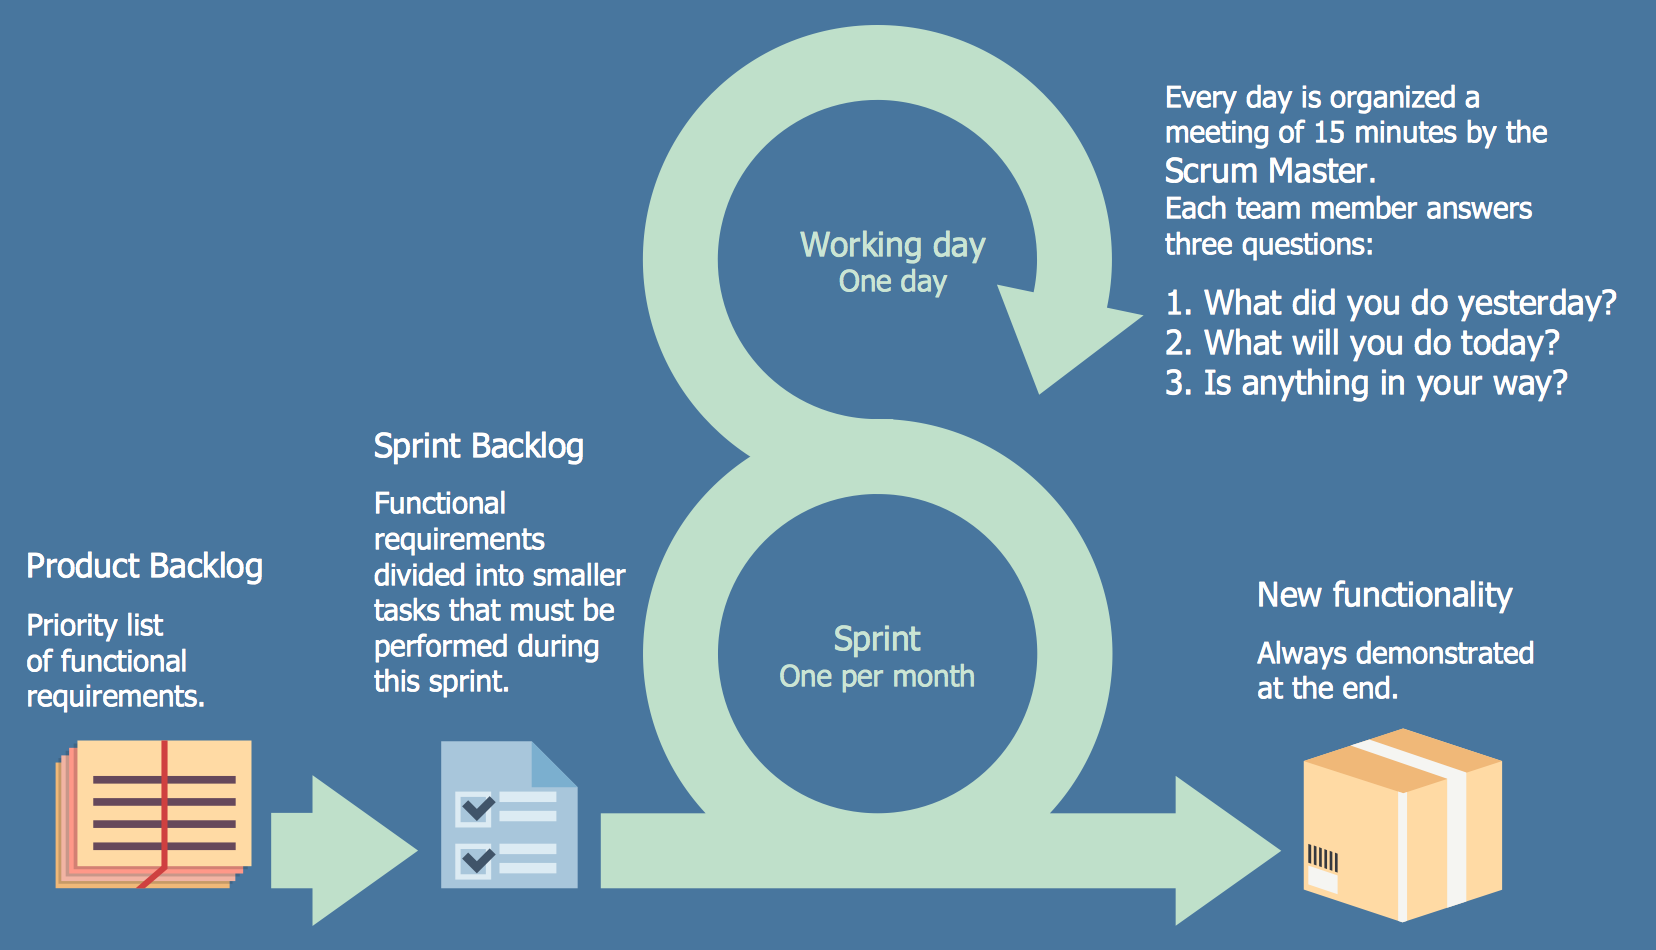
\includegraphics[scale=0.25]{../media/scrum-workflow.png} \\
    \textit{Quelle:} \href{https://www.conceptdraw.com/How-To-Guide/scrum-workflow}{conceptdraw}
\end{center}
Das vom Product Owner erstellte Product Backlog wird im \textbf{Sprint Backlog} in kleinere Aufgaben aufgeteilt, die während dieser Arbeitseinheit erledigt werden sollen. Eine solche Arbeitseinheit dauert in der Regel zwischen 2 und 4 Wochen und wird \textbf{Sprint} genannt. Die Entwickler einigen sich darauf, wie viel des Product Backlogs in diesem Sprint abgearbeitet werden kann  \\
Wichtig dabei ist aber, dass nicht jeder der Entwickler die gesamte Zeit alleine vor sich hinwerkelt, sondern es gibt an jedem Arbeitstag ein Meeting (der \textbf{Daily Scrum}) an dem die drei oben abgebildeten Fragen beantwortet werden, frei übersetzt:
\begin{enumerate}
    \item Was ist gestern passiert?
    \item Was wird heute passieren?
    \item Gibt es Probleme?
\end{enumerate}
Diese Besprechungen sollen \textbf{kurz} und \textbf{effizient} sein - was sich in der Praxis häufig als schwierig heraustellt (hört man zumindest..). Am Ende eines Sprints gibt es - idealerweise - eine neue Version der Software bzw. ein neues Feature, das getestet werden kann im sogenannten \textbf{Sprint Review}. Hier sind häufig auch Kunden und insbesondere Anwender beteiligt. Der Sprint wird mit dann mit der \textbf{Sprint-Retrospektive} beendet - im Wesentlichen eine Team-interne Besprechung, inwiefern in Zukunft effizienter und effektivergearbeitet werden kann. \\

\textit{Hinweis:} Der ganze Prozess kann natürlich noch viel detaillierter dargestellt werden und es gibt auch noch deutlich mehr Details, für uns genügt aber dieser Überblick! \\

\color{purp} \textbf{Bei uns:} \color{black} In der Schule benötigen wir die volle Pracht des Scrum-Workflows natürlich nicht, dennoch sollen Kernpunkte dieser Arbeitsweise in die Projektarbeit mit einfließen (Details und Beispiele dazu im Kapitel \q{Das Projekt}):
\begin{itemize}
    \item Das Product Backlog (also die Beschreibung des zu entwickelnden Programs) wird in Form von \textbf{User Stories} zusammengestellt. Eine User Story ist dabei eine möglichst genaue Beschreibung in Alltagssprache, was das Programm können soll. 
    \item Die Sprint-Dauer wird auf 1 bis 1,5 Wochen verkürzt, da das gesamte Projekt voraussichtlich nur eine Dauer von etwa 8 Wochen haben wird. 
    \item Der Daily Scrum ist nicht möglich, es soll aber mindestens in jeder Unterrichtsstunde eine Besprechung des Teams geben - also nicht nur \q{basteln}.
    \item Auch der Sprint Review soll möglichst während der Unterrichtszeit stattfinden (voraussichtlich Donnerstags, Ende der 3. Stunde) - um Tests auch mit nicht-Teammitgliedern zu ermöglichen. 
    \item Vereinbarungen (also z.B. die User Stories) oder Implementierungsdetails sollen \textbf{schriftlich} festgehalten werden. Auch die Priorisierung - also was soll zuerst implementiert werden - soll deutlich gemacht werden. 
\end{itemize}


\end{document}